
%% bare_conf.tex
%% V1.4
%% 2012/12/27
%% by Michael Shell
%% See:
%% http://www.michaelshell.org/
%% for current contact information.
%%
%% This is a skeleton file demonstrating the use of IEEEtran.cls
%% (requires IEEEtran.cls version 1.8 or later) with an IEEE conference paper.
%%
%% Support sites:
%% http://www.michaelshell.org/tex/ieeetran/
%% http://www.ctan.org/tex-archive/macros/latex/contrib/IEEEtran/
%% and
%% http://www.ieee.org/

%%*************************************************************************
%% Legal Notice:
%% This code is offered as-is without any warranty either expressed or
%% implied; without even the implied warranty of MERCHANTABILITY or
%% FITNESS FOR A PARTICULAR PURPOSE! 
%% User assumes all risk.
%% In no event shall IEEE or any contributor to this code be liable for
%% any damages or losses, including, but not limited to, incidental,
%% consequential, or any other damages, resulting from the use or misuse
%% of any information contained here.
%%
%% All comments are the opinions of their respective authors and are not
%% necessarily endorsed by the IEEE.
%%
%% This work is distributed under the LaTeX Project Public License (LPPL)
%% ( http://www.latex-project.org/ ) version 1.3, and may be freely used,
%% distributed and modified. A copy of the LPPL, version 1.3, is included
%% in the base LaTeX documentation of all distributions of LaTeX released
%% 2003/12/01 or later.
%% Retain all contribution notices and credits.
%% ** Modified files should be clearly indicated as such, including  **
%% ** renaming them and changing author support contact information. **
%%
%% File list of work: IEEEtran.cls, IEEEtran_HOWTO.pdf, bare_adv.tex,
%%                    bare_conf.tex, bare_jrnl.tex, bare_jrnl_compsoc.tex,
%%                    bare_jrnl_transmag.tex
%%*************************************************************************

% *** Authors should verify (and, if needed, correct) their LaTeX system  ***
% *** with the testflow diagnostic prior to trusting their LaTeX platform ***
% *** with production work. IEEE's font choices can trigger bugs that do  ***
% *** not appear when using other class files.                            ***
% The testflow support page is at:
% http://www.michaelshell.org/tex/testflow/



% Note that the a4paper option is mainly intended so that authors in
% countries using A4 can easily print to A4 and see how their papers will
% look in print - the typesetting of the document will not typically be
% affected with changes in paper size (but the bottom and side margins will).
% Use the testflow package mentioned above to verify correct handling of
% both paper sizes by the user's LaTeX system.
%
% Also note that the "draftcls" or "draftclsnofoot", not "draft", option
% should be used if it is desired that the figures are to be displayed in
% draft mode.
%
\documentclass[journal]{IEEEtran}
% Add the compsoc option for Computer Society conferences.
%
% If IEEEtran.cls has not been installed into the LaTeX system files,
% manually specify the path to it like:
% \documentclass[conference]{../sty/IEEEtran}





% Some very useful LaTeX packages include:
% (uncomment the ones you want to load)


% *** MISC UTILITY PACKAGES ***
%
%\usepackage{ifpdf}
% Heiko Oberdiek's ifpdf.sty is very useful if you need conditional
% compilation based on whether the output is pdf or dvi.
% usage:
% \ifpdf
%   % pdf code
% \else
%   % dvi code
% \fi
% The latest version of ifpdf.sty can be obtained from:
% http://www.ctan.org/tex-archive/macros/latex/contrib/oberdiek/
% Also, note that IEEEtran.cls V1.7 and later provides a builtin
% \ifCLASSINFOpdf conditional that works the same way.
% When switching from latex to pdflatex and vice-versa, the compiler may
% have to be run twice to clear warning/error messages.






% *** CITATION PACKAGES ***
%
%\usepackage{cite}
% cite.sty was written by Donald Arseneau
% V1.6 and later of IEEEtran pre-defines the format of the cite.sty package
% \cite{} output to follow that of IEEE. Loading the cite package will
% result in citation numbers being automatically sorted and properly
% "compressed/ranged". e.g., [1], [9], [2], [7], [5], [6] without using
% cite.sty will become [1], [2], [5]--[7], [9] using cite.sty. cite.sty's
% \cite will automatically add leading space, if needed. Use cite.sty's
% noadjust option (cite.sty V3.8 and later) if you want to turn this off
% such as if a citation ever needs to be enclosed in parenthesis.
% cite.sty is already installed on most LaTeX systems. Be sure and use
% version 4.0 (2003-05-27) and later if using hyperref.sty. cite.sty does
% not currently provide for hyperlinked citations.
% The latest version can be obtained at:
% http://www.ctan.org/tex-archive/macros/latex/contrib/cite/
% The documentation is contained in the cite.sty file itself.

\usepackage{hyperref}




% *** GRAPHICS RELATED PACKAGES ***
%
\ifCLASSINFOpdf
  % \usepackage[pdftex]{graphicx}
  % declare the path(s) where your graphic files are
  % \graphicspath{{../pdf/}{../jpeg/}}
  % and their extensions so you won't have to specify these with
  % every instance of \includegraphics
  % \DeclareGraphicsExtensions{.pdf,.jpeg,.png}
\else
  % or other class option (dvipsone, dvipdf, if not using dvips). graphicx
  % will default to the driver specified in the system graphics.cfg if no
  % driver is specified.
  % \usepackage[dvips]{graphicx}
  % declare the path(s) where your graphic files are
  % \graphicspath{{../eps/}}
  % and their extensions so you won't have to specify these with
  % every instance of \includegraphics
  % \DeclareGraphicsExtensions{.eps}
\fi
% graphicx was written by David Carlisle and Sebastian Rahtz. It is
% required if you want graphics, photos, etc. graphicx.sty is already
% installed on most LaTeX systems. The latest version and documentation
% can be obtained at: 
% http://www.ctan.org/tex-archive/macros/latex/required/graphics/
% Another good source of documentation is "Using Imported Graphics in
% LaTeX2e" by Keith Reckdahl which can be found at:
% http://www.ctan.org/tex-archive/info/epslatex/
%
% latex, and pdflatex in dvi mode, support graphics in encapsulated
% postscript (.eps) format. pdflatex in pdf mode supports graphics
% in .pdf, .jpeg, .png and .mps (metapost) formats. Users should ensure
% that all non-photo figures use a vector format (.eps, .pdf, .mps) and
% not a bitmapped formats (.jpeg, .png). IEEE frowns on bitmapped formats
% which can result in "jaggedy"/blurry rendering of lines and letters as
% well as large increases in file sizes.
%
% You can find documentation about the pdfTeX application at:
% http://www.tug.org/applications/pdftex
\usepackage{graphicx}
\usepackage{listings} %for code snippets
\usepackage[tableposition=top]{caption}


% *** MATH PACKAGES ***
%
\usepackage[cmex10]{amsmath}
% A popular package from the American Mathematical Society that provides
% many useful and powerful commands for dealing with mathematics. If using
% it, be sure to load this package with the cmex10 option to ensure that
% only type 1 fonts will utilized at all point sizes. Without this option,
% it is possible that some math symbols, particularly those within
% footnotes, will be rendered in bitmap form which will result in a
% document that can not be IEEE Xplore compliant!
%
% Also, note that the amsmath package sets \interdisplaylinepenalty to 10000
% thus preventing page breaks from occurring within multiline equations. Use:
%\interdisplaylinepenalty=2500
% after loading amsmath to restore such page breaks as IEEEtran.cls normally
% does. amsmath.sty is already installed on most LaTeX systems. The latest
% version and documentation can be obtained at:
% http://www.ctan.org/tex-archive/macros/latex/required/amslatex/math/





% *** SPECIALIZED LIST PACKAGES ***
%
%\usepackage{algorithmic}
% algorithmic.sty was written by Peter Williams and Rogerio Brito.
% This package provides an algorithmic environment fo describing algorithms.
% You can use the algorithmic environment in-text or within a figure
% environment to provide for a floating algorithm. Do NOT use the algorithm
% floating environment provided by algorithm.sty (by the same authors) or
% algorithm2e.sty (by Christophe Fiorio) as IEEE does not use dedicated
% algorithm float types and packages that provide these will not provide
% correct IEEE style captions. The latest version and documentation of
% algorithmic.sty can be obtained at:
% http://www.ctan.org/tex-archive/macros/latex/contrib/algorithms/
% There is also a support site at:
% http://algorithms.berlios.de/index.html
% Also of interest may be the (relatively newer and more customizable)
% algorithmicx.sty package by Szasz Janos:
% http://www.ctan.org/tex-archive/macros/latex/contrib/algorithmicx/




% *** ALIGNMENT PACKAGES ***
%
%\usepackage{array}
% Frank Mittelbach's and David Carlisle's array.sty patches and improves
% the standard LaTeX2e array and tabular environments to provide better
% appearance and additional user controls. As the default LaTeX2e table
% generation code is lacking to the point of almost being broken with
% respect to the quality of the end results, all users are strongly
% advised to use an enhanced (at the very least that provided by array.sty)
% set of table tools. array.sty is already installed on most systems. The
% latest version and documentation can be obtained at:
% http://www.ctan.org/tex-archive/macros/latex/required/tools/


% IEEEtran contains the IEEEeqnarray family of commands that can be used to
% generate multiline equations as well as matrices, tables, etc., of high
% quality.




% *** SUBFIGURE PACKAGES ***
%\ifCLASSOPTIONcompsoc
%  \usepackage[caption=false,font=normalsize,labelfont=sf,textfont=sf]{subfig}
%\else
%  \usepackage[caption=false,font=footnotesize]{subfig}
%\fi
% subfig.sty, written by Steven Douglas Cochran, is the modern replacement
% for subfigure.sty, the latter of which is no longer maintained and is
% incompatible with some LaTeX packages including fixltx2e. However,
% subfig.sty requires and automatically loads Axel Sommerfeldt's caption.sty
% which will override IEEEtran.cls' handling of captions and this will result
% in non-IEEE style figure/table captions. To prevent this problem, be sure
% and invoke subfig.sty's "caption=false" package option (available since
% subfig.sty version 1.3, 2005/06/28) as this is will preserve IEEEtran.cls
% handling of captions.
% Note that the Computer Society format requires a larger sans serif font
% than the serif footnote size font used in traditional IEEE formatting
% and thus the need to invoke different subfig.sty package options depending
% on whether compsoc mode has been enabled.
%
% The latest version and documentation of subfig.sty can be obtained at:
% http://www.ctan.org/tex-archive/macros/latex/contrib/subfig/




% *** FLOAT PACKAGES ***
%
%\usepackage{fixltx2e}
% fixltx2e, the successor to the earlier fix2col.sty, was written by
% Frank Mittelbach and David Carlisle. This package corrects a few problems
% in the LaTeX2e kernel, the most notable of which is that in current
% LaTeX2e releases, the ordering of single and double column floats is not
% guaranteed to be preserved. Thus, an unpatched LaTeX2e can allow a
% single column figure to be placed prior to an earlier double column
% figure. The latest version and documentation can be found at:
% http://www.ctan.org/tex-archive/macros/latex/base/


%\usepackage{stfloats}
% stfloats.sty was written by Sigitas Tolusis. This package gives LaTeX2e
% the ability to do double column floats at the bottom of the page as well
% as the top. (e.g., "\begin{figure*}[!b]" is not normally possible in
% LaTeX2e). It also provides a command:
%\fnbelowfloat
% to enable the placement of footnotes below bottom floats (the standard
% LaTeX2e kernel puts them above bottom floats). This is an invasive package
% which rewrites many portions of the LaTeX2e float routines. It may not work
% with other packages that modify the LaTeX2e float routines. The latest
% version and documentation can be obtained at:
% http://www.ctan.org/tex-archive/macros/latex/contrib/sttools/
% Do not use the stfloats baselinefloat ability as IEEE does not allow
% \baselineskip to stretch. Authors submitting work to the IEEE should note
% that IEEE rarely uses double column equations and that authors should try
% to avoid such use. Do not be tempted to use the cuted.sty or midfloat.sty
% packages (also by Sigitas Tolusis) as IEEE does not format its papers in
% such ways.
% Do not attempt to use stfloats with fixltx2e as they are incompatible.
% Instead, use Morten Hogholm'a dblfloatfix which combines the features
% of both fixltx2e and stfloats:
%

\usepackage{float}
%\usepackage{dblfloatfix}
% The latest version can be found at:
% http://www.ctan.org/tex-archive/macros/latex/contrib/dblfloatfix/


\usepackage{enumitem}


% *** PDF, URL AND HYPERLINK PACKAGES ***
%
%\usepackage{url}
% url.sty was written by Donald Arseneau. It provides better support for
% handling and breaking URLs. url.sty is already installed on most LaTeX
% systems. The latest version and documentation can be obtained at:
% http://www.ctan.org/tex-archive/macros/latex/contrib/url/
% Basically, \url{my_url_here}.




% *** Do not adjust lengths that control margins, column widths, etc. ***
% *** Do not use packages that alter fonts (such as pslatex).         ***
% There should be no need to do such things with IEEEtran.cls V1.6 and later.
% (Unless specifically asked to do so by the journal or conference you plan
% to submit to, of course. )


% correct bad hyphenation here
\hyphenation{op-tical net-works semi-conduc-tor}


\begin{document}
%
% paper title
% can use linebreaks \\ within to get better formatting as desired
% Do not put math or special symbols in the title.
\title{Face Image Morphing (May 2017)}


% author names and affiliations
% use a multiple column layout for up to three different
% affiliations
\author{Conrad~Appel$^1$, Danton~Zhao$^2$, Logan~Campbell$^3$\\ 
		Lyle School of Engineering, Computer Engineering$^1$, Electrical Engineering$^{2,3}$\\
		Southern Methodist University
        }
        
%\author{\IEEEauthorblockN{\textbf{Danton Zhao}}
%\IEEEauthorblockA{Lyle School of Engineering\\Electrical Engineering\\
%Southern Methodist University\\
%Dallas, Texas 75275-0100\\
%Email: dantonz@smu.edu}}

%~\IEEEmembership{Member,~IEEE,}
%        John~Doe,~\IEEEmembership{Fellow,~OSA,}
%        and~Jane~Doe,~\IEEEmembership{Life~Fellow,~IEEE}%

% conference papers do not typically use \thanks and this command
% is locked out in conference mode. If really needed, such as for
% the acknowledgment of grants, issue a \IEEEoverridecommandlockouts
% after \documentclass

% for over three affiliations, or if they all won't fit within the width
% of the page, use this alternative format:
% 
%\author{\IEEEauthorblockN{Michael Shell\IEEEauthorrefmark{1},
%Homer Simpson\IEEEauthorrefmark{2},
%James Kirk\IEEEauthorrefmark{3}, 
%Montgomery Scott\IEEEauthorrefmark{3} and
%Eldon Tyrell\IEEEauthorrefmark{4}}
%\IEEEauthorblockA{\IEEEauthorrefmark{1}School of Electrical and Computer Engineering\\
%Georgia Institute of Technology,
%Atlanta, Georgia 30332--0250\\ Email: see http://www.michaelshell.org/contact.html}
%\IEEEauthorblockA{\IEEEauthorrefmark{2}Twentieth Century Fox, Springfield, USA\\
%Email: homer@thesimpsons.com}
%\IEEEauthorblockA{\IEEEauthorrefmark{3}Starfleet Academy, San Francisco, California 96678-2391\\
%Telephone: (800) 555--1212, Fax: (888) 555--1212}
%\IEEEauthorblockA{\IEEEauthorrefmark{4}Tyrell Inc., 123 Replicant Street, Los Angeles, California 90210--4321}}




% use for special paper notices
%\IEEEspecialpapernotice{(Invited Paper)}




% make the title area
\maketitle

% no keywords
\begin{abstract}
In this paper, we propose an implementation of Facial Image Morphing using openCV. Our framework uses the detection of facial features in an image and then warps and adjusts the pixel intensity values determined by a predefined alpha value. Alpha is a value between 0 and 1 that determines the presence of each original image in the morphed image.
\end{abstract}



% For peer review papers, you can put extra information on the cover
% page as needed:
% \ifCLASSOPTIONpeerreview
% \begin{center} \bfseries EDICS Category: 3-BBND \end{center}
% \fi
%
% For peerreview papers, this IEEEtran command inserts a page break and
% creates the second title. It will be ignored for other modes.
\IEEEpeerreviewmaketitle



\section{Introduction}
\IEEEPARstart{A}{t the} simplest level, Image morphing is simply the blending of pixels of image $I$ and $J$ to create $M$ using: 
\begin{align} \label{eq:1}
M(x,y) &= (1-\alpha)I(x,y) + \alpha*J(x,y) 
\end{align}
\begin{align*}
0 &\leq \alpha \leq 1   
\end{align*}
When $\alpha = 0$ , $M$ will be identical to $I$, and when $\alpha =1$, it will look like $J$. This simplistic method will blend the two images, but the faces will most likely not be aligned and this will result in a blurry mess of image $M$ \newline 
% You must have at least 2 lines in the paragraph with the drop letter
% (should never be an issue)

Thus, we must establish pixel correspondence between images $I$ and $J$. Only then can we calculate the pixel locations in $M$. The $x$ and $y$ locations in $M$ can be represented with:
\begin{align}\label{eq:2}
X_M &= (1-\alpha)X_I + \alpha*X_J\\ \label{eq:3} 
Y_M &= (1-\alpha)Y_I + \alpha*Y_J   
\end{align}

Equation \hyperref[eq:1]{(\ref{eq:1})} is then applied to the shifted pixels to obtain our morphed image.

% An example of a floating figure using the graphicx package.
% Note that \label must occur AFTER (or within) \caption.
% For figures, \caption should occur after the \includegraphics.
% Note that IEEEtran v1.7 and later has special internal code that
% is designed to preserve the operation of \label within \caption
% even when the captionsoff option is in effect. However, because
% of issues like this, it may be the safest practice to put all your
% \label just after \caption rather than within \caption{}.
%
% Reminder: the "draftcls" or "draftclsnofoot", not "draft", class
% option should be used if it is desired that the figures are to be
% displayed while in draft mode.
%
%\begin{figure}[!t]
%\centering
%\includegraphics[width=2.5in]{myfigure}
% where an .eps filename suffix will be assumed under latex, 
% and a .pdf suffix will be assumed for pdflatex; or what has been declared
% via \DeclareGraphicsExtensions.
%\caption{Simulation Results.}
%\label{fig_sim}
%\end{figure}

% Note that IEEE typically puts floats only at the top, even when this
% results in a large percentage of a column being occupied by floats.


% An example of a double column floating figure using two subfigures.
% (The subfig.sty package must be loaded for this to work.)
% The subfigure \label commands are set within each subfloat command,
% and the \label for the overall figure must come after \caption.
% \hfil is used as a separator to get equal spacing.
% Watch out that the combined width of all the subfigures on a 
% line do not exceed the text width or a line break will occur.
%
%\begin{figure*}[!t]
%\centering
%\subfloat[Case I]{\includegraphics[width=2.5in]{box}%
%\label{fig_first_case}}
%\hfil
%\subfloat[Case II]{\includegraphics[width=2.5in]{box}%
%\label{fig_second_case}}
%\caption{Simulation results.}
%\label{fig_sim}
%\end{figure*}
%
% Note that often IEEE papers with subfigures do not employ subfigure
% captions (using the optional argument to \subfloat[]), but instead will
% reference/describe all of them (a), (b), etc., within the main caption.


% An example of a floating table. Note that, for IEEE style tables, the 
% \caption command should come BEFORE the table. Table text will default to
% \footnotesize as IEEE normally uses this smaller font for tables.
% The \label must come after \caption as always.
%
%\begin{table}[!t]
%% increase table row spacing, adjust to taste
%\renewcommand{\arraystretch}{1.3}
% if using array.sty, it might be a good idea to tweak the value of
% \extrarowheight as needed to properly center the text within the cells
%\caption{An Example of a Table}
%\label{table_example}
%\centering
%% Some packages, such as MDW tools, offer better commands for making tables
%% than the plain LaTeX2e tabular which is used here.
%\begin{tabular}{|c||c|}
%\hline
%One & Two\\
%\hline
%Three & Four\\
%\hline
%\end{tabular}
%\end{table}


% Note that IEEE does not put floats in the very first column - or typically
% anywhere on the first page for that matter. Also, in-text middle ("here")
% positioning is not used. Most IEEE journals/conferences use top floats
% exclusively. Note that, LaTeX2e, unlike IEEE journals/conferences, places
% footnotes above bottom floats. This can be corrected via the \fnbelowfloat
% command of the stfloats package.


\section{Image Morphing Technique}
\subsection{Landmark Detection}
	First, to find each corresponding points in images I and J, we used Dlib, a general-purpose C++-based toolkit, to detect facial landmarks. Dlib creates a bag of features using a Histogram of Ordered Gradients, then classifies using a sliding window detection. Dlib’s model was trained to return 68 distinct points at specific points on a face (such as on the corners of the lips, the edge of the face, and more). In addition to Dlib’s facial landmarks, we added anchor points to the corners of the images because we also want to morph the pieces of the image that fall outside of the main face.

\subsection{Subdivision}
Using our set of points, we subdivide the image using Delaunay Triangulation. This algorithm aims to create triangle subdivisions between all of the points while maximizing the minimum angle present in any triangle. By doing this maximization, we create the “fattest” triangles possible and minimize “sliver” triangles - ones that are extremely thin. Each of these triangles are represented within the application as sets of 3 point coordinates each. 
We also create a separate subdivision for each triangle to use within the next step - a rectangular subsection of the original image that is cropped using a bounding box around the triangle. Using this subdivision proves beneficial because many library functions expect a simple two dimensional array to perform operations on (such as cv2.wiarpAffine(), as described below).

\subsection{Warping}
To warp or blend the two images we must use equations \hyperref[eq:2]{(\ref{eq:2})} and \hyperref[eq:3]{(\ref{eq:3})} to locate the pixels in image M. Then we calculate the affine transform using OpenCV’s getAffineTransform. This will map the three corners of a triangle in image I or J to a corresponding triangle in M. Then we must warp all of the pixels inside each triangle to M. This is achieved using the function warpAffine. It must be noted that warpAffine only takes in an image and not a triangle, so we had to create a bounding box for each triangle and then create a triangular mask using fillConvexPoly.
Finally after some fine-tuning to hide the seams, the images can be blended using varying values of $\alpha$.

\subsection{Find Corresponding Points}
\begin{enumerate}[label=\alph*)]
\item Dlib
\begin{enumerate}[label=\roman*)]
	\item dlib.get$\_$frontal$\_$face$\_$detector() to find a bounding box over a face
	\begin{enumerate}[label=\arabic*)]
		\item Uses sliding window classifier over a histogram of gradients pyramid
	\end{enumerate}
	\item dlib.shape$\_$predictor() to find “key-points” within the bounding box
	\begin{enumerate}[label=\arabic*)]
		\item Model trained over the HELEN dataset for facial feature detection
	\end{enumerate}
\end{enumerate}
\end{enumerate}

\subsection{Delaunay Triangulation}
\begin{enumerate}[label=\alph*)]
\item Algorithm used to maximize the minimum necessary angle within triangles within points (no “slivers”)
\item Used cv2.Subdiv2D class and .getTriangleList()
\begin{enumerate}[label=\roman*)]
	\item This handled the triangulation algorithm for us
	\item Returns a list of sets of 3 points (x $\&$ y coordinates)
	\item We only had to clean up the results a little bit
	\begin{enumerate}[label=\arabic*)]
		\item Discard triangles that extended beyond the image
		\item Establish the one-to-one correspondence between each image's triangles
	\end{enumerate}
\end{enumerate}
\end{enumerate}
\subsection{Warping Images}
\begin{enumerate}[label=\alph*)]
\item Iterate through all available triangles
\item Calculate the affine transformations from I$\rightarrow$M and J$\rightarrow$M
\item
	\begin{align}
		\begin{bmatrix}
			x_i' \\ y_i'
		\end{bmatrix}
		&= Affine\_transform \cdot
		\begin{bmatrix}
			x_i \\ y_i \\ 1
		\end{bmatrix}
	\end{align}
\item Use warpAffine to apply the affine transform
\item Apply triangle mask to only retrieve morphed triangle
\begin{figure}[H]
	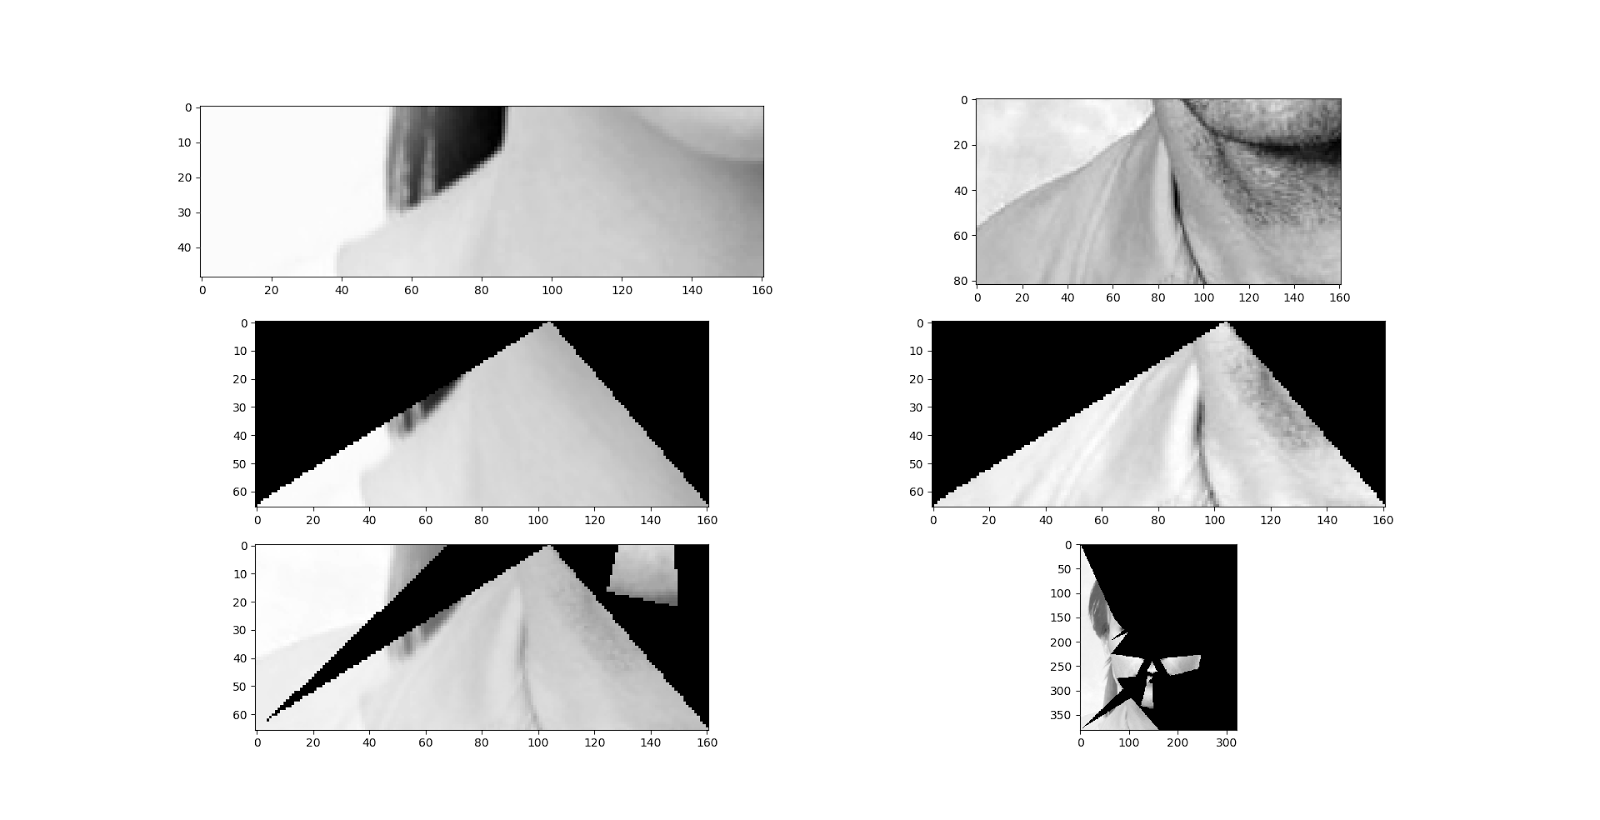
\includegraphics[width = \linewidth]{triangles}
	\caption{Masked Triangles}
\end{figure}
\end{enumerate}

\subsection{GIF Creation}
A GIF, at its most basic, is a series of static images joined and played in series.  It’s possible to use imageio Python package’s ability to compile this information and output to a GIF format. After passing in an N-dimensional NumPy array of images, a back-and-forth effect demonstrates the morphing from image I to J as well as from J to I. The reverse playback can be created by appending the reverse of the image array to itself. Because each frame in a GIF can have an independent duration, a longer pause at the start and end frames should be created to emphasize each original image. Also, a compression in the number of available colors using the GIF’s format ability will reduce the image file size.

\subsection{Server}
	An in-class demonstration is a desirable goal and it is important that the server works as seamlessly as possible which includes a fast result. Generating the independent frames of the GIF is a highly-parallelizable and independent job. Thus, we spawn subprocesses, whose number depends on how many logical cores are available, to which frame-generation is offloaded.
\begin{enumerate}[label=\alph*)]
\item Simple REST Server based on CherryPy with two endpoints
\begin{enumerate}[label=\roman*)]
	\item /static returns static files (HTML, JS, CSS, etc)
	\item /upload accepts two images and redirects the user to a static GIF file after calling the image$\_$morpher
\end{enumerate}

\item Performance:
\begin{enumerate}[label=\roman*)]
	\item Since an in-class demo was an end goal, we wanted to make sure it worked as seamlessly as possible - this included getting a fast result.
	\item Generating the independent frames of the GIF is a highly-parallelizable and independent job. Thus, we spawn subprocesses (number depending on how many logical cores are available) to which frame-generation is offloaded
\end{enumerate}
\end{enumerate}


\section{Results}
	The generated GIF results in a seamless transition from image I to J using varying values of alpha to morph the two images. Examples of this transition can be seen in Appendix B. While image morphing and GIF generation seems to perform well on a PC, users may have difficulty with results when accessing the server on a mobile device. If an image depicts a face with glasses, this may also cause problems with the program.  


\section{Conclusion}
In this paper, we provide a framework for implementing Facial Image Morphing using Python, Dlib, and OpenCV. By varying the value of alpha we are able to create an array of images that will demonstrate a transition from image I to J and can be viewed as a GIF. This is a proof of concept that if we are able to create one-to-one delaunay triangles in two images, seamless morphing is possible.

\section{Appendix A: Code}
See \url{https://github.com/conradhappeliv/imagemorpher} for the full code-base and instructions on running.


% conference papers do not normally have an appendix


% use section* for acknowledgement
%\section*{Acknowledgment}








% trigger a \newpage just before the given reference
% number - used to balance the columns on the last page
% adjust value as needed - may need to be readjusted if
% the document is modified later
%\IEEEtriggeratref{8}
% The "triggered" command can be changed if desired:
%\IEEEtriggercmd{\enlargethispage{-5in}}

% references section

% can use a bibliography generated by BibTeX as a .bbl file
% BibTeX documentation can be easily obtained at:
% http://www.ctan.org/tex-archive/biblio/bibtex/contrib/doc/
% The IEEEtran BibTeX style support page is at:
% http://www.michaelshell.org/tex/ieeetran/bibtex/
%\bibliographystyle{IEEEtran}
% argument is your BibTeX string definitions and bibliography database(s)
%\bibliography{IEEEabrv,../bib/paper}
%
% <OR> manually copy in the resultant .bbl file
% set second argument of \begin to the number of references
% (used to reserve space for the reference number labels box)
\begin{thebibliography}{1}

\bibitem{}
http://docs.opencv.org/2.4/modules/imgproc/doc/geometric$\_$transformations.html
?highlight=getaffinetransform$\#$warpaffine

\bibitem{}
http://docs.opencv.org/2.4/modules/imgproc/doc/geometric$\_$transformations.html
$\#$getaffinetransform

\bibitem{}
http://dlib.net/imaging.html$\#$get$\_$frontal$\_$face$\_$detector

\bibitem{}
http://dlib.net/imaging.html$\#$shape$\_$predictor

\bibitem{}
http://imageio.readthedocs.io/en/latest/userapi.html$\#$imageio.mimwrite

\bibitem{}
https://github.com/

\end{thebibliography}

\section{Appendix C: Examples}
\begin{figure*}[!t]\label{fig:merge}
	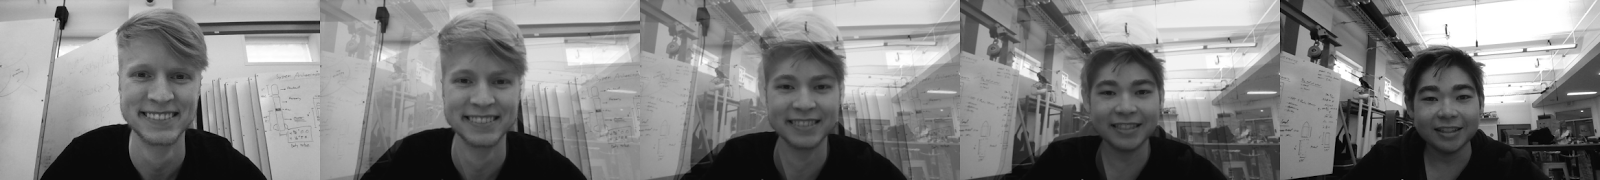
\includegraphics[width = \linewidth]{sample1}
	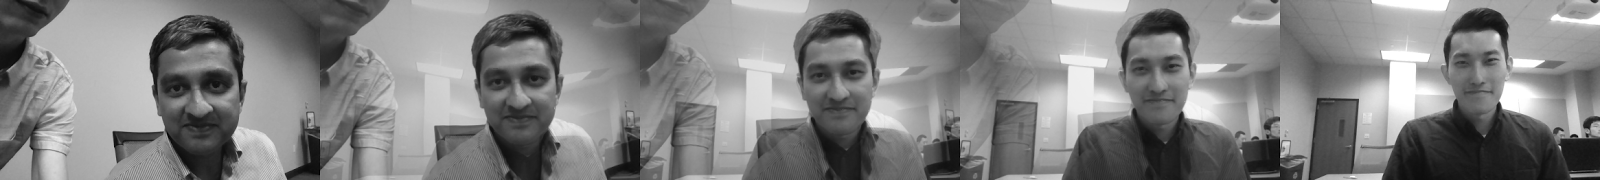
\includegraphics[width = \linewidth]{sample2}
	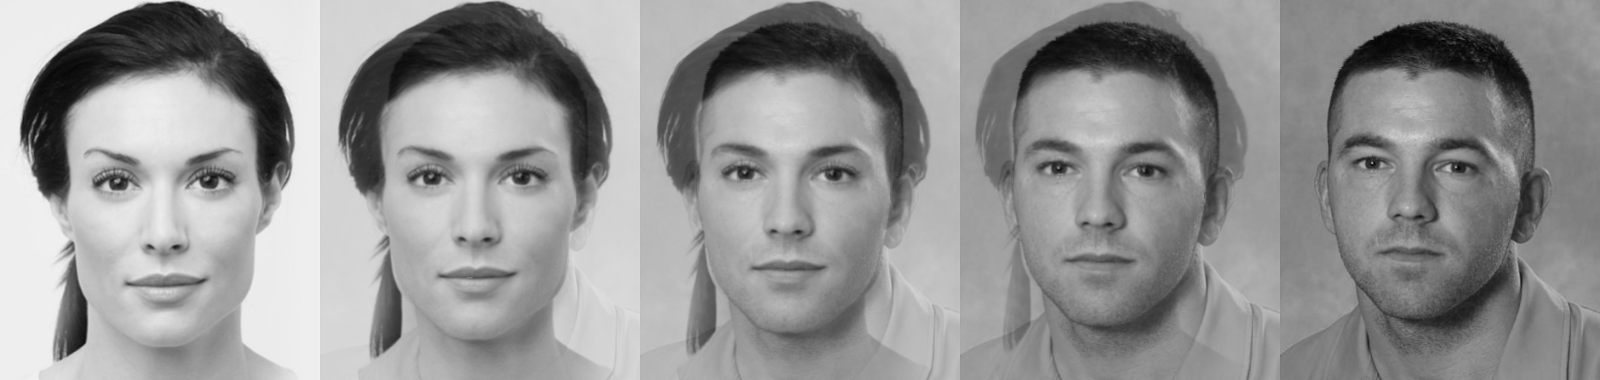
\includegraphics[width = \linewidth]{sample3}
	\caption{Sample Merge Sequences}
The following code was used to generate these images
\end{figure*}

\begin{figure*}[!t]\label{fig:code}
\begin{lstlisting}[language=Python]
face1 = io.imread('data/face5.jpg')
face2 = io.imread('data/face6.jpg')
face1gray = cv2.cvtColor(face1, cv2.COLOR_RGB2GRAY)
face2gray = cv2.cvtColor(face2, cv2.COLOR_RGB2GRAY)
res = None
for key, amt in enumerate([0, .25, .5, .75, 1]):
   r = morph(face1, face2, amt, False)
   if res is None:
       res = np.zeros((r.shape[0], r.shape[1]*5), np.float32)
   res[:, key*r.shape[1]:(key+1)*r.shape[1]] = r
from PIL import Image
img = Image.fromarray(res, 'F')
img = img.convert('RGB')
img.save('out.png')

#To generate the 6-tiled pic up above:
plt.subplot(3, 2, 1)
plt.imshow(subimg1, cmap=plt.cm.gray)
plt.subplot(3, 2, 2)
plt.imshow(subimg2, cmap=plt.cm.gray)
plt.subplot(3, 2, 3)
plt.imshow(warped1*mask, cmap=plt.cm.gray)
plt.subplot(3, 2, 4)
plt.imshow(warped2*mask, cmap=plt.cm.gray)
combined = newimg_sq + (alpha_blend * mask)[:newimg_sq.shape[0], :newimg_sq.shape[1]]
plt.subplot(3, 2, 5)
plt.imshow(combined, cmap=plt.cm.gray)
newimg[bb_morph[1]:bb_morph[1] + bb_morph[3], bb_morph[0]:bb_morph[0] + bb_morph[2]] 
	= newimg_sq + (alpha_blend * mask)[:newimg_sq.shape[0], :newimg_sq.shape[1]]
plt.subplot(3, 2, 6)
plt.imshow(newimg, cmap=plt.cm.gray)
plt.show()

\end{lstlisting}
\end{figure*}

% that's all folks
\end{document}


